\documentclass[12pt]{report}
\usepackage{crackerjack}

% Additional packages not handled by crackerjack.sty
\usepackage{amsmath, amsfonts, amsthm, amssymb}
\usepackage{float}
\usepackage{wrapfig}
\usepackage{cleveref}
\usepackage{mathtools}
\usepackage{verbatim}
\usepackage{appendix}
\usepackage{cancel}
\usepackage{derivative}

% ── Custom chapter command ────────────────────────────────────
\newcommand{\mychapter}[2]{%
    \setcounter{chapter}{#1}%
    \setcounter{section}{0}%
    \chapter*{#2}%
    \addcontentsline{toc}{chapter}{#2}%
}

\begin{document}

% ── 1. Title page ─────────────────────────────────────────────
\maketitle

% ── 2. Abstract — own page, vertically centred ───────────────
\begin{abstract}
\textit{The Hitchhiker's Guide to the Galaxy} is, among other things,
a book designed to help its reader navigate a universe that is
confusing, chaotic, and occasionally hostile. This guide has far more
modest ambitions: to help you remain at least somewhat functional while
staring at a block of ciphertext that appears to have been designed
specifically to ruin your evening. If there is one thing worth
remembering throughout the rest of this guide, it is the same advice
printed in large, friendly letters on the cover of the
\textit{Hitchhiker's Guide}:
\href{https://en.wikipedia.org/wiki/Phrases_from_The_Hitchhiker%27s_Guide_to_the_Galaxy#Don't_Panic}{\textbf{DON'T PANIC}}.
\end{abstract}

% ── 3. Preface (not in TOC, no header) ───────────────────────
\chapter*{What this guide is (and isn't)}
\thispagestyle{plain}

This is not a guide on how to break codes.

There are plenty of places you can go if what you want is the
mechanics: how to run frequency analysis, how to implement a
hill-climb attack, or which button to press next in Python. If
that's what you're looking for, this guide will probably feel a bit
frustrating.

This is a guide on how to be a codebreaker. Or at least, a guide I
wish I had when I first started.

It's about what to do before you know what cipher you're even looking
at. How to think when nothing makes sense yet, how to recognise
progress when there is no readable plaintext in sight, and how to stay
functional and vaguely sane when you're stuck, because at some point,
you absolutely will be.

Codebreaking, especially with something like the National Cipher
Challenge, is very rarely a neat sequence of steps. More often than
not, it's long periods of uncertainty sprinkled with small insights
that only feel obvious in hindsight.

Most of the difficulty in codebreaking comes from uncertainty like not
knowing where to start, or whether you're making progress, and not
knowing whether the idea you're attached to is actually helping.

In short, if you've ever stared at a block of ciphertext and thought
to yourself, \textit{`I have no idea what I'm doing'}, then you're in
the right place.

% ── 4. Table of contents ─────────────────────────────────────
\tableofcontents
\thispagestyle{plain}

% ── 5. Chapters ──────────────────────────────────────────────

\mychapter{1}{Being Stuck}
\epigraph{Not all those who wander are lost}
{\textit{J.R.R. Tolkien}}

\section{Transition from Familiar Problems}

Most problems you have probably met before come with some kind of scaffolding.

In mathematics, you are given an equation and expected to apply a known method. In physics, you identify the model, plug in the numbers, and hope the units work out in your favour. Even when a problem is difficult, there is usually a sense of what kind of solution it requires. You may not immediately know how to proceed, but you recognise the structure of the task. You know what tools are available, what progress might look like, and roughly how far you are from an answer.

\section{Why Codebreaking Feels Different}

Codebreaking does not usually begin with that same clarity.

When you first encounter a difficult cipher, nobody hands you a tidy label saying this is a \texttt{substitution cipher} or this one is \texttt{Vigenère but with a twist}\footnote{I must say this isn't strictly true. Depending on how generous Harry and Jodie are feeling, they might let a small hint or two slip before the first deadline!}. There is no signpost telling you whether the symbols represent letters, groups of letters, sounds, numbers, or something much weirder.

Instead of being guided towards a method, you are presented with something that has been deliberately designed to conceal its structure, so you have to work out what the problem even is before you can begin solving it. This is, unfortunately, much less glamorous than it sounds and often involves staring at repeated symbols until your brain starts assigning emotional significance to bigrams.

Without a clear framework, it becomes very easy to panic slightly and start throwing methods at the problem in quick succession. You try one thing. It doesn't work. You try another. Then another. And after a while, you begin to get the horrible creeping sense that the cipher is not impossible, exactly, but that it has somehow become personal.

\section{The Point of the Challenge}

It is very tempting, at first, to think of codebreaking as an exercise in applying techniques efficiently. But if the goal were simply to run frequency analysis, implement known algorithms, or write a program that could quickly decode a given cipher, then much of the difficulty would disappear. Once the method is identified, the rest becomes largely mechanical.

Competitions like the Cipher Challenge go beyond this. The difficulty, and the point, lies in working out what to do in the first place. It lies in recognising structure, forming hypotheses, and deciding which ideas are worth pursuing. 


\section{On Feeling 'Stuck'}

In most areas, being stuck has a fairly obvious meaning: you have reached a point where you do not know how to continue.

In codebreaking, I think the meaning is more subtle. The difficulty is in knowing which method is worth trying, or whether any of them apply at all. And given that the whole point of the challenge is to figure out what kind of problem you are solving in the first place, that experience is not a sign something has gone wrong. It is just what the beginning looks like.

If you expect yourself to recognise the correct approach immediately, any delay starts to feel like a mistake. It usually isn't. Being stuck, in this sense, means you do not yet know what kind of problem you are solving. Which, if you think about it, is exactly where you are supposed to be.


\begin{figure}
    \centering
    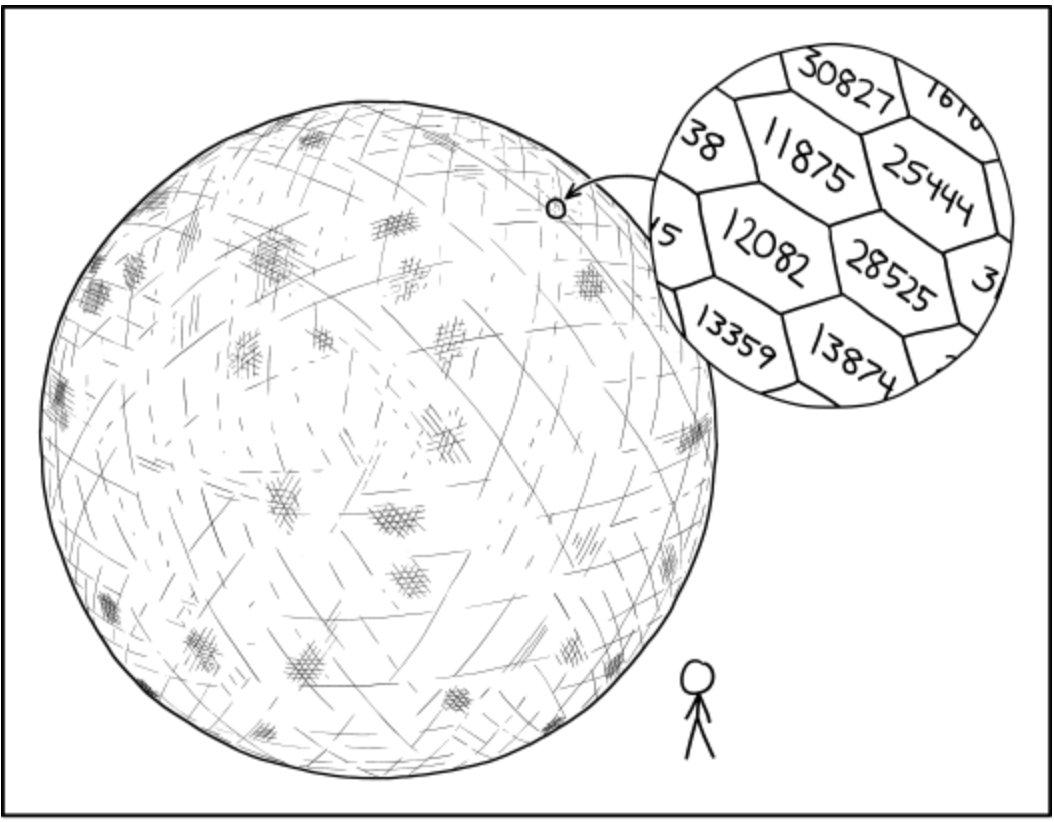
\includegraphics[width=0.5\linewidth]{xkcd/d65536.png}
    \caption{\textbf{\href{https://www.explainxkcd.com/wiki/index.php/2626:_d65536}{2626: d65536}}}
\end{figure}


\mychapter{2}{Redefining Progress}
% really wanna talk about marginal gains when I first read itn James Clear's book, cite that here - https://jamesclear.com/marginal-gains
\epigraph{Success is the product of daily habits--not once-in-a-lifetime transformations}
{\textit{James Clear}}


\section{Marginal Gains}

In elite sport, there is an idea referred to as \textbf{marginal gains}\footnote{I first read about this in James Clear's Atomic Habits, an excerpt from which can be found \textbf{\href{https://jamesclear.com/marginal-gains}{\textit{here}}}}. The principle is simple: instead of looking for one large breakthrough, you focus on making many small improvements. Each small change on its own might seem insignificant, but together, they compound. 

One of the most well-known examples of this comes from British cycling. In the years leading up to their Olympic dominance, the team became almost absurdly committed to improving everything by tiny amounts. They monitored training, nutrition, recovery, sleep, equipment, even the things that seemed too small to be worth bothering with. What stood out was not the scale of any single improvement, but the accumulation of many small ones. 


\section{Why Progress Doesn’t Feel Like Progress} 

The difficulty is that small improvements don't tend to announce themselves. There is no intermediate output to confirm you are moving in the right direction, and without that feedback, it is easy to interpret the absence of a solution as the absence of progress.

If progress is defined only as having solved the cipher, then everything before that point starts to feel like failure. Which is a terrible definition, not least because it means you can spend hours doing genuinely intelligent work and still come away feeling like you achieved nothing. Ignoring real improvements because no single one seems large enough to count is exactly the marginal gains mistake. 

I say that not from a position of great wisdom, but as someone who has absolutely stared at ciphertext for an hour, made several useful observations, and then convinced myself I was getting nowhere because none of them had yet turned into plaintext.


\section{Narrowing the Problem}

At the start of a cipher, there are usually many possible interpretations. The text could represent letters, numbers, symbols, or groups. It could be the result of a simple substitution, a transposition, or one of those ciphers that makes you briefly question whether language itself was a mistake. Without additional information, these possibilities can feel equally plausible.

When you notice that certain patterns repeat in a consistent way, you begin to rule out some explanations. When the number of distinct symbols is too high or too low for a particular method, that method becomes less likely. When a hypothesis fails to produce consistent results, it can be set aside.

Over time, this process narrows the range of possibilities as each step removes options until what remains is manageable enough to analyse more directly.


\section{A More Useful Definition} 

Instead of asking: \textit{Have I solved the problem? }Try asking: \textit{Do I understand the problem better than I did before?}

If the answer is yes even in the slightest, then progress has been made. You may not yet have a solution, or may not even be close to one, but if you have ruled out possibilities, identified structure, or clarified your assumptions, then you have moved forward.

This shift in perspective is important because it allows you to value the marginal gains and the incremental steps that lead to understanding rather than focusing only on the final result. 


\begin{figure}[H]
    \centering
    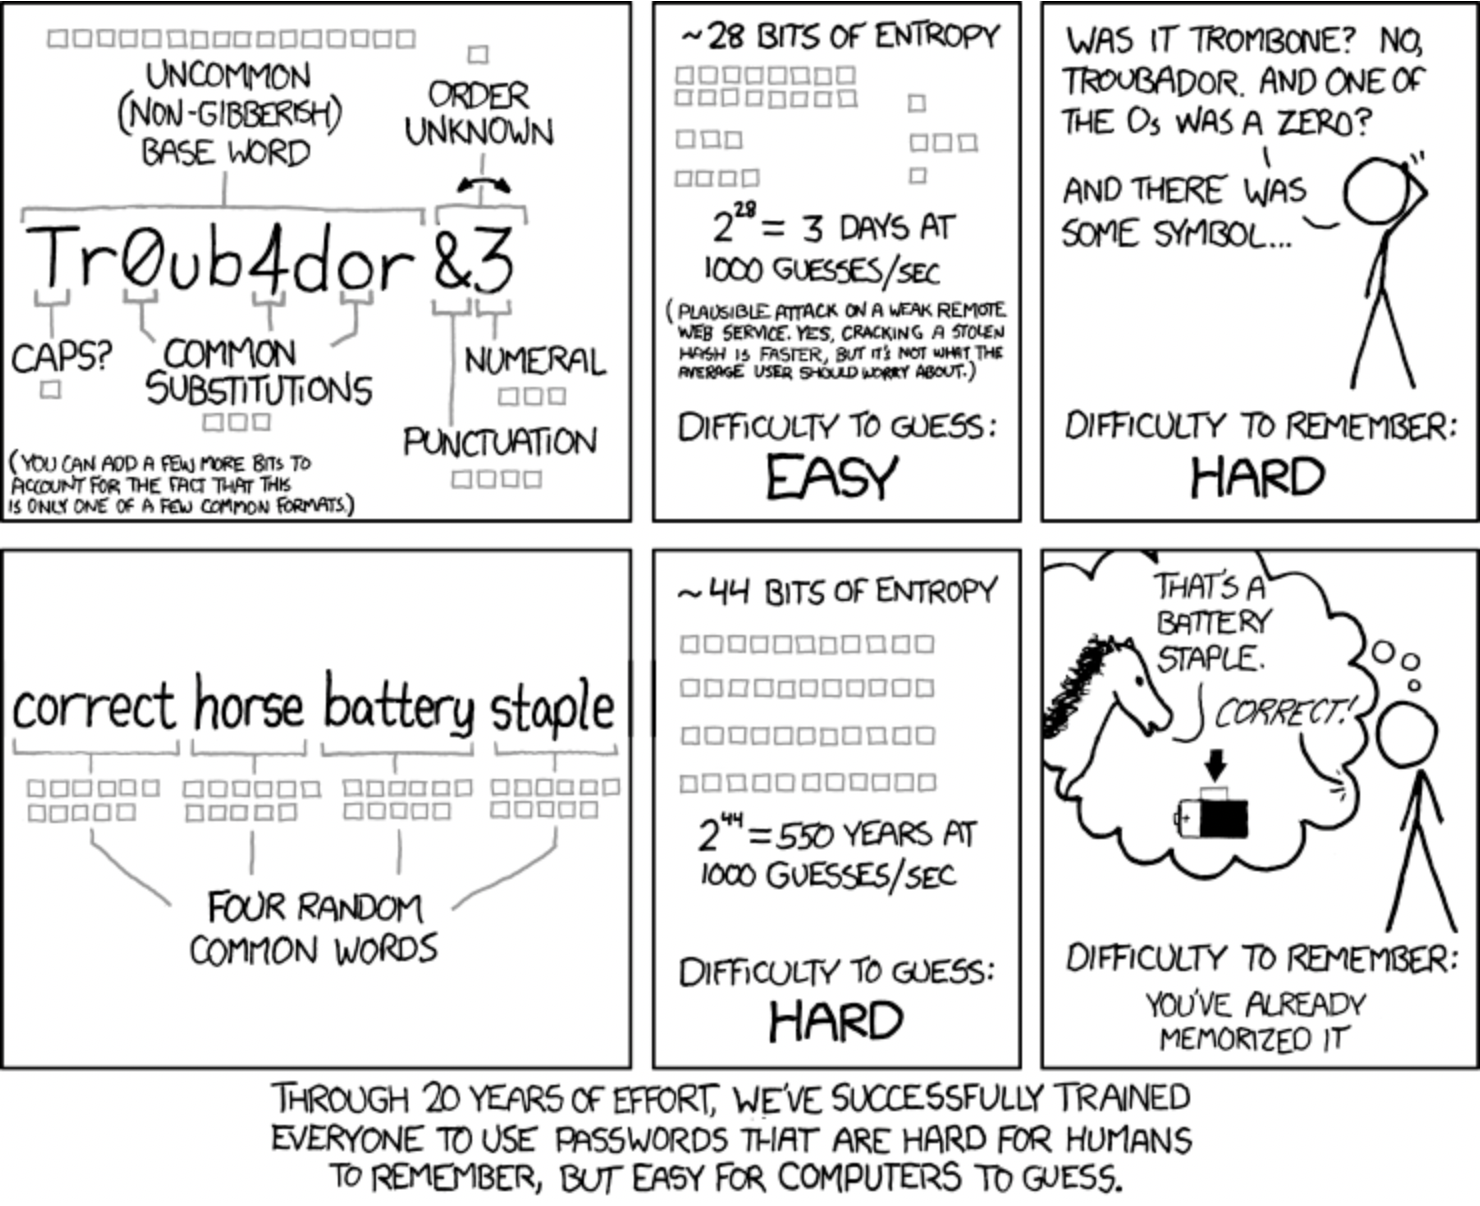
\includegraphics[width=0.5\linewidth]{xkcd/passwordStrength.png}
    \caption{\textbf{\href{https://www.explainxkcd.com/wiki/index.php/936:_Password_Strength}{936: Password Strength}}}
\end{figure}

\mychapter{3}{The Starting Line}
\epigraph{Slow is smooth, and smooth is fast}
{\textit{Military proverb}}

\section{Speed vs Accuracy}

As much as this challenge rewards speed, it also rewards accuracy. In the later challenges especially, I often found that acting too quickly meant committing to an idea before the problem had been properly understood. When an initial idea fails, it is easy to move on to another, and then another again, without ever fully engaging with the structure of the cipher itself.

A more effective approach might be to first pause. After all, there is a reason races begin with \textit{On Your Marks... Get Set... Go!} and not just someone yelling \textit{GO!} at a group of already stressed people. The pause is not separate from the start, it's part of the start. It gives you a second to settle, to look ahead, to position yourself, and to begin with some sense of direction rather than pure adrenaline.

Codebreaking is no different. So before attempting to solve anything, it helps to take a step back and look carefully at what is actually in front of you. At this stage, your goal is not to crack the cipher, but to understand what you're dealing with.

\section{What Is Actually There}

When you look at the ciphertext as it is, ask questions about what you can see. Think of going through steps of a mental flowchart to problem solving 

Some questions you might want to consider could be: 
\begin{itemize}
    \item What characters appear? 
    \item How many distinct characters are there? 
    \item Do certain patterns in the text repeat? 
    \item Are there deliberate spaces in the text? 
\end{itemize}

These questions do not require any specialised knowledge as they are less about applying techniques, and more about paying attention to the information that is already present.


\section{Defining the Unit}

One of the most important questions you can ask yourself early on is: \textbf{What is one unit of this ciphertext? }

It might be natural to assume that each character corresponds to a letter. But ciphers are under no obligation to be that cooperative. A single symbol might represent a letter, or a pair of letters, or a number, or a code. Maybe the groupings of such symbols or characters only make sense when they appear in a certain pattern. 

For example, in Morse code, individual dots and dashes are not letters. Only when they are grouped in the correct way do they form meaningful units, so treating each symbol independently would not lead to a solution. And if you get the unit wrong, you can spend a very long time being impressively wrong in a highly committed way.

Recognising the correct unit is not always immediate. But simply knowing that this is a question worth asking can save you from making assumptions too early, which is one of the more common ways to accidentally make your own life harder.

\section{Asking Better Questions}

If there’s anything I’ve learned, it’s that quality of your thinking is determined by the quality of the questions you ask.

At the beginning of a cipher, it is easy to focus on questions that are too specific about the type of cipher. But those questions assume that you already understand the problem well enough to classify it.

More useful questions are broader and more structural such as: 
\begin{itemize}
    \item What patterns are present? 
    \item What is and isn't consistent? 
    \item What assumptions am I making? 
    \item What would have to be true for this to work? 
\end{itemize}

Notice how the questions above don't have quick answers, but they do guide your attention in a more productive direction in the sense that they help you build a clearer picture of the problem before committing to a particular approach.

The purpose of the starting line is not to immediately produce an answer, but to begin understanding the problem in a structured way. By observing carefully, questioning assumptions, and resisting the urge to act too quickly, you create the conditions for meaningful progress later on.

\begin{figure}
    \centering
    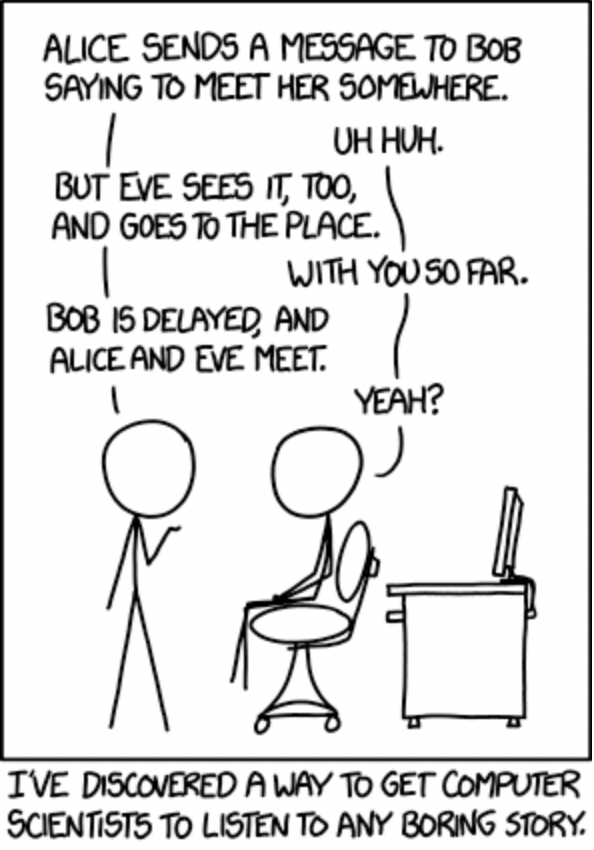
\includegraphics[width=0.5\linewidth]{xkcd/protocol.png}
    \caption{\textbf{\href{https://www.explainxkcd.com/wiki/index.php/1323:_Protocol}{1323: Protocol}}}
\end{figure}

\mychapter{4}{Abandoning Ideas}
\epigraph{It is a capital mistake to theorize before one has data. Insensibly one begins to twist facts to suit theories, instead of theories to suit facts.}
{\textit{Sir Arthur Conan Doyle}}

\section{The Difficulty of Letting Go}

There is a well-known tendency in business decision making called the \textbf{\textit{\href{https://en.wikipedia.org/wiki/Sunk_cost}{sunk cost fallacy}}}. Once time, effort or resources have been invested into something, it becomes much harder to away even when continuing is no longer the best option. 

A classic example is watching a film you are not enjoying. Half an hour in, you realise it is not very good. The plot is weak, the dialogue is unbearable, and at least one character appears to have been written by someone who has never met another human being. But instead of turning it off, you keep watching, because you have already spent thirty minutes on it and the whole thing is only ninety.

The same thing could happen in codebreaking. After spending a long time developing an idea, testing it and trying to make it work, it becomes difficult to let go. The time you have invested starts to feel like a reason to continue even when the evidence might no longer support it. 

Every year that I have competed in the challenge, this has been one of the most difficult things to deal with. Not because the problem was particularly complex, but because I was then faced with a choice: continue with an idea that feels promising, or abandon it and return to uncertainty.

\section{Why We Hold On}

It's very natural to become attached to an idea once you have invested enough of yourself into it. And by `yourself', I don't just mean your time. I also mean your hope, concentration, and sense that this has all been leading somewhere. 

The more work you have done, the more difficult it becomes to let go. Each small success reinforces the belief that you're close to a solution, even when the overall picture does not quite fit. An idea that is `almost perfect' can be quite dangerous because it creates the illusion that you are only one step away from solving the problem. 

There is also a tendency to adjust the problem to fit the idea. If something does not align perfectly, it can be tempting to treat it as an exception, or to assume that it will make sense later. But over time, this can lead to increasingly complicated explanations that are difficult to justify, but equally difficult to abandon.

\section{When an Idea just isn’t Working}

Letting go of an idea becomes easier when you know what to look for. This is genuinely difficult, but gets easier with time and practice and patience. 

Some common signs that an idea may not be useful include:
\begin{itemize}
    \item The explanation only works for part of the ciphertext
    \item You need to summon exceptions to make it fit
    \item Small inconsistencies are being ignored or explained away
    \item The reasoning becomes more complicated over time, rather than simpler
\end{itemize}

A useful principle here is that good explanations tend to simplify the problem. So if an idea requires increasing effort to maintain, it is often a sign that it is not the right one. 

\section{Returning to the Problem}

After abandoning an idea, it is important to return to the problem itself, rather than immediately searching for a replacement. 

Go back to the ciphertext. Look again at what is actually there. Revisit the observations that still hold. Ask yourself what remains true even now that your favourite idea has collapsed dramatically in front of you.

By returning to the structure of the problem, you allow new ideas to emerge from what you can observe, rather than from what you hope might work.

Again, abandoning an idea does not mean starting again from nothing. Even if a particular approach does not lead to a solution, the process of exploring it may still have produced useful information. You may have ruled out certain structures, identified patterns that remain consistent, or clarified which assumptions do not hold.

These point is that these insights remain valuable. The goal here is not to avoid being wrong. That would be both impossible and extremely boring. The goal is to be wrong in ways that sharpen your understanding, to fail usefully, to let the bad ideas die without dragging you down with them.

\mychapter{5}{Using Context}
%Basically  - give real life examples from WW2 or something on why context is insanely useful when codebreaking 
%Cribbing is underrated - it’s not just a fancy term for guesswork, it’s strategic guesswork. It’s one way how the allies broke the Enigma. 
%How to think like the code setter - think aobut final challenges… not gonna repeat themselves.. often based on the theme. Theme of cards in 2025, needle telegraph in 2024. 
%I think the cipher challenge does a really good of including context. The keys for ciphers are often relate to the story or the title in some way. Exploit that fact,  make note of those tiny details, they’re insanely important. Look at the pattern.. some ciphers repeat every year, others not very often. 
%In terms of context- also look at like length of solution and other things at the end. Make sure lunch matches that of the cipher text if it as one to one thing? 
% https://en.wikipedia.org/wiki/Cryptanalysis_of_the_Enigma


\section{War and Cribs}

During WW2, much of the Allied effort\footnote{This became extremely important when it came to \textbf{\href{https://en.wikipedia.org/wiki/Cryptanalysis_of_the_Enigma}{breaking the Enigma}}} in breaking encrypted messages relied on \textbf{cribs}, which is a just a fancy word for fragments of plaintext that were expected to appear in the decoded messages. 

The important thing to note is that these were not random guesses. Messages often followed predictable formats. Certain phrases like weather reports, routine communications, and repeated structures all provided opportunities to make educated assumptions about what the plaintext might contain. By aligning these expected fragments with intercepted ciphertext, codebreakers were able to recover information about the encryption process. This essentially provided a way into systems that would have otherwise been extremely difficult to analyse directly. 

The point being, these breakthroughs did not come purely from analysing symbols in isolation. 


\section{Choosing Cribs}

As mentioned before, a crib is not chosen at random, it is based on reasonable expectations about what the plaintext might contain. 

And where can we these expectations within the challenge? Context. 

Fortunately for National Cipher Challenge, no context is accidental. The ciphers are designed with intention around a theme/story, which means that the plaintext is not going to be arbitrary. So in many cases, we can infer a lot of information about content in the ciphertexts from context on the site, especially the \texttt{Case Files} section. Other examples include: 

\begin{itemize}
    \item Titles may hint at key(s) or type of cipher used 
    \item Recurring named figures across the challenges 
    \item Specific dates or years hinting towards historic events
    \item Certain themes being reflected in the structure of the ciphertext. Eg: telegraph machine in 2024(10B) and playing cards in 2025(10B) 
\end{itemize}

You almost want to think like the code-setter and ask yourself questions that make you think about why information is presented in the way that it is. Remember that everything you need to solve the problem is given to you. 


\section{Using Context Cautiously}

While context is incredibly powerful, it must be used with caution. An educated guess that fits the theme could potentially be a red-herring. So remember sunk cost fallacy and challenge any assumptions you make. 

Context also plays a useful role when you've acquired a solution. For instance: 

\begin{itemize}
    \item Does the length of your solution match the ciphertext (only if a one-to-one mapping is expected, but you get the idea) 
    \item Does the solution make sense within the theme of the challenge 
    \item Does the solution have any missing/incomplete sections? 
\end{itemize}

Remember that spaces don't matter in your solution as all spaces and punctuation are removed from submissions when they are checked.  







\mychapter{6}{Teamwork}
%There is value is teamwork. Having competed the challenge in both individually and in different  teams over the years, there are pros and cons to both. A good team can lift your ability, not so great teammates just leave it when challenges get tough, but that’s fine.. at leats you know you’ want stick with it. I’ve experienced both sides. Having a supportive team as well as one that just left and didn’t do anything. 
%Also wanna talk about how I didn’t do any programming, but being part of a team meant I could learn from others. It’s a good team building exercise, good way to know people, especially if you’ve ended up changing schools for sixth form or something which is what I ended up doing. Had to form a new team. Something about the experience of shared suffering… people bringing different set of skills which can be useful. Some are very good ate rogramming.. others at recognising what works and doesn’t… good to bounce back ideas form each other.. but also can lead to argument and falling out… that’s tough. So just, look after each other. 
%Other resources you could have as a team…we had a shared GitHub reporsitoeyr we worked on over the summer and writing solutions to ciphers that were common in the competition. 
%Team captain login- remember that only that account that submit solutions, so if you team captain wants it might be a good idea to share that with the team so that others can submit the solution in case they can’t get hold of the captain. 


\section{Methods of Competing}

Having competed in the competition both individually and as part of different teams overs, I've had some experience of both sides. 

Working alone can be focused as you move at your own pace, follow your own ideas and don't have to coordinate with anyone else. But it can also be isolating at times, especially when you get stuck. 

A good team on the other hand can lift your ability. It gives your different perspectives, methods of thinking, and people to bounce ideas off. At the same time, not every works efficiently and sometimes when challenges get tough, people drift away. So if you ever find yourself left alone towards the end when you started of with a team, rest assured, it's quite normal. From my experience, being the only left taught me the kind of person I wanted to be in a team, namely someone who stays, contributes, and stick with it when things get tough.

Having joined a new school for sixth form, I had the fun change of joining a new team from scratch. Working together on the cipher challenge later turned out to be one of the easiest ways to get to know people. It's genuinely an amazing experience to work together to solve a problem that no one fully understands. 

\section{Learning from Each Other}

One of the biggest advantages of working in a team is the opportunity to learn from one another. 

For instance, when I first started competing in the NCC, I could barely code. But working alongside friends who shared this enthusiasm for problem-solving created an environment in which I saw my confidence in coding improve. At the start of my sixth form year, I had just over a year of coding experience and could identify most commonly used ciphers in the challenge, but I didn't really see myself as the `coding person'\footnote{The only Python programs I recall writing were an IOC calculator and a simple Vigenère cipher solver for a known key}. Yet, through the process of contributing to our team's shared GitHub repository, I found myself working on annealing and modified Playfair ciphers. Whether it was optimising the hill climb parameters for various programs, or spotting a silly inequality error in the quadgram evaluation block, the shared teamwork made even the most daunting ciphers feel achievable.

At the same time, programming isn't the only skill that matters. Some people are amazing at coding and automating processes, whereas others are better at spotting patterns, recognising when something doesn't quite it, and knowing when to move onto another idea. 

A good team brings all of these strengths together.

\section{Shared Thinking}

An idea that seems convincing in your own head can start to fall apart when you try to explain it out loud. On the other hand, someone else might take the same idea and see something you didn't. There's a lot of scope for progress from conversations with teammates. 

There's also something to be said for the experience itself. The shared frustration, the moments where nothing makes sense, and the occasional breakthrough when something suddenly clicks. That shared experience is a big part of what makes this competition memorable. 

Teamwork is not always smooth. People work and think at different speeds and sometimes ideas clash and disagreements happen. When things get difficult, it's easy for communication to break down. 

It helps to remember that everyone is working towards the same common goal. So taking a step back, listening to each other and being willing to let go of your own initial ideas to intake new information can make a big difference. 

\section{Working Practically}

Listed below are some things that helped our team work more efficiently, and I hope you might find something useful here: 

\begin{itemize}
    \item Sharing Progress - it can be useful to have something like a team Discord server or any group chat so that you can communicate and keep each other updated with progress 
    \item Divide and Explore - different people can test different ideas at the same time which can speed up the process of ruling things out 
    \item Shared resources - my team kept a shared GitHub repo where we stored all our scripts and solutions to most common ciphers. Having  a shared codebase can be very useful in the long term and make later challenges easier to approach  
    \item Team captain login - since only the 'Team Captain' account can submit solutions, it might be worth to make sure more than one person has access to it in case the team captain is unavailable 
\end{itemize}


\mychapter{7}{Tools and Resources}
Chapter 7 — Tools and Resources
%Why forum is GOATED 
%There are lots of online tools on solving ciphers.. competition rules forbid using that.. but you can have a look at them to learn??? 
%In terms of importing your way to victory… 


To be honest, I learned Python during GCSEs, but just the basics to get me a good grade. Having never done any programming before that, most of my coding experience came from writing solutions for the cipher challenge problems, which in turn helped me in A-Level and just improving thinking skills in general. Am at uni now and most of the things I’ve learned is thanks to the experienced gained by taking part in this competition.  

I might be biased, but I genuinely think the best way to learn is by just doing projects. Every now and then I start a new maths/coding project, not necessarily with the intention of always finishing it, but I almost always end up learning a lot in the process. So pick something you enjoy and do it for fun, not just because you think you “should”. As much as I loved writing code for solving challenges, there were definitely times when it became stressful, and if you find that happening, it’s usually a sign you should switch things up for a bit. Sometimes that means working on a different problem, and sometimes it means doing something completely different. At one point I picked up crocheting, and I vividly remember crocheting while debugging my A-Level code because I was getting so frustrated with a program that refused to run. Weirdly, that kind of break actually helped more than staring at the screen ever did.

There are plenty of good books and resources which the far more experienced here will be happy to recommend, but I’ve mostly relied on learning by searching things as I go, because I personally find that big books can be overwhelming when you don’t yet know what’s relevant. There’s a very high chance that whatever problem you’re stuck on has been hit by someone before (funnily enough this is true in both programming and life…). I’ve also been grateful to have friends and people around me who were there to help, so I’d suggest finding a similar community for yourself. It makes a massive impact being around people who share a similar goal to you than doing everything by yourself. When I first started programming, I never imagined I’d be able to solve the kinds of problems I can today. It can be really daunting at first, especially when you’re looking at other people’s code and it all feels incomprehensible, but you have to keep things in perspective and trust the learning process, it genuinely does add up over time! 


\mychapter{8}{The Long Game}
% Refine from the long post on \texttt{10B} on Forum + other stuff 

\section{\texttt{Challenge 10B}}

If this is your first year, \texttt{Challenge 10B} is the final and most difficult challenge of the season. If you've done this before, you already know the deal. 

One of the most difficult things I find with \texttt{10B} every year, apart from the cipher itself, is knowing when to take a break. 

In the midst of chaotic, spiralling ideas on how to crack the final cipher, it’s so easy to fall into that trap of `I’m so close… just a bit longer…' and then 5 hours later your eyes hurt, brain’s fried, and you’re resisting the urge to throw your laptop out the window. 

It feels completely counterintuitive, but stepping away really does help. And even knowing that, I still find it hard to move away when I'm in the zone. 

Over time, I've found a few things that helped me reset and come back with a clearer head. None of these solve the cipher, but they make it much easier to think when you return: 

\textbf{Write Down Everything You Know}\\
Every hour or just pick a timeframe, jot down everything you’ve figured out about the cipher, even the obvious stuff, especially the obvious stuff. Key lengths, repeated n-grams, letter positions, ciphertext arrangement, possible cribs, structure. 

It’s easy to feel like you’re not making much progress, but when you see it on paper, it’s surprising how much you’ve actually uncovered, and it helps track progress. 

\textbf{Have a snack}\\
The brain burns a ridiculous amount of energy when you’re problem-solving. As I’ve been told many times in training: food is fuel.

\textbf{Check in with your team if you have one}\\
It's easy to disappear into your own rabbit hole of ideas so it’s always useful take a moment to sync and share weird hunches, and remind each other to take breaks as well.

\textbf{Setting Expectations}\\
Setting expectations at home if need be. My family is always made well aware that I will be busy during cipher challenge season, especially towards the end so they know what to or not to expect from me. I find that this definitely does reduce some background stress 

\textbf{Stepping Away}\\
Slightly unconventional, but I have a hoodie I only wear when working on the cipher challenge\footnote{Sadly it doesn’t have any actual powers, but having a dedicated codebreaking hoodie does make me feel extra geeky}. 

When I take a break, I physically change out of it. It sounds silly but that very act of changing the hoodie helps me switch mental gears and actually rest. As much as we all love the challenge, I’m sure we all have other things (including food and sleep) that need getting done and I just found that having a physical reminder helped me compartmentalise

\textbf{Sleep}\\
I don't think I need to explain this further. Sleep is good for you, so please remember to sleep at a somewhat sensible time.


\section{Sticking With It}

Having done the cipher challenge for five years, my only real regret was not sticking with \texttt{10B} till the end in my second year. 

I gave up too early and convinced I was going nowhere after working on it for just over a day, only to see others break through with just a bit more persistence. 

What I’ve learned since then is that hints do come, but you’ve got to have patience. They’re mostly be subtle or buried under obscure forum comments, or phrased in a way that only makes sense after you’ve cracked it. 

\section{Celebrating the Little Wins}

It's very easy to let the whole thing feel overwhelming. So try and celebrate the little victories. Remember that marginal gains eventually add up. 

Yes, winning is great, but it's not all about the winning. It sounds cliché to say \textit{value the process over the outcome} but it's actually true. With any performance comes pressure. You start wanting to do well, to keep up and get things right. And slowly, without realising, that pressure can suck the joy out of the experience. 

Don't let the desire to do well take away the reason you started in the first place; don't let the need to perform rip off the curiosity, enjoyment and satisfaction of figuring something out for yourself. 

It's quite funny but I think that if you’re annoyed at a cipher, that’s kind of amazing in itself. 

It means you’ve found something that you care about. Something that's gripped your attention so much that you're willing to struggle with and keep thinking even when it would be easier to stop, and that's rare. 

Most people go through life bored by what they do because let’s be real, if a bunch of weirdly spaced letters and numbers are making you want to throw your keyboard across the room, maybe that’s just be a sign you’ve found something worth fighting with (and for), and that’s a beautiful thing. 

Remember that the feeling of finally solving it is always worth the storm of frustration and patience and mild existential crisis or whatever mix of emotions it takes to get there. 

\section{More than Just Codebreaking}

If anything, this challenge teaches you more than just codebreaking. 

Over the holidays especially, cipher challenge has been escapism in the best sense for me. There's something deeply comforting about knowing that no matter what else is going on, there's always a cipher waiting to be cracked, and a community engaged in doing the same.

And in many ways, the lessons you learn during the competition stay with you as well. Some of the most difficult things I’ve faced over the past few months were made more manageable because of what I learned while struggling with the challenges. Patience, persistence, and the willingness to keep trying different ideas even when the solution isn’t obvious are skills that apply far beyond cryptography. 


\end{document}